\documentclass[conference]{IEEEtran}
\RequirePackage{cite}
\RequirePackage{amsmath,amssymb,amsfonts}
\RequirePackage{algorithmic}
\RequirePackage{graphicx}
\RequirePackage{textcomp}
\RequirePackage{xcolor}
\RequirePackage{hyperref}
\RequirePackage{csquotes}
\setkeys{Gin}{width=0.4\textwidth}
\def\BibTeX{{\rm B\kern-.05em{\sc i\kern-.025em b}\kern-.08em
    T\kern-.1667em\lower.7ex\hbox{E}\kern-.125emX}}
\begin{document}
\title{Autonomous Sailboating}
\author{Andrew~Fearing, Neelay~Junnarkar,  Hamza~Kamran~Khawaja}
\maketitle


\begin{abstract}
Sailboat

\end{abstract}


\section{Introduction}
\subsection{Motivation}
Sailboats have the potential to go on long-term missions at sea. They need actuators only for the rudder and sail, and so they can be solar powered
\subsection{Applications}
\subsection{Sailboats}

\section{Related Work}


\section{Methods}
Coding and Algorithms
\section{Results}
\begin{figure}
    \centering
    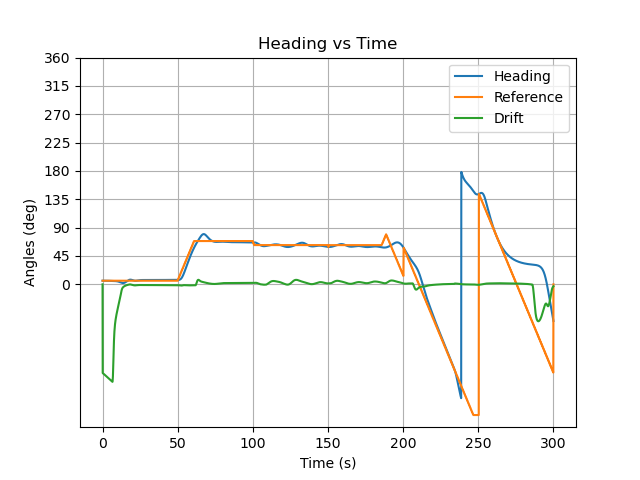
\includegraphics{documents/final_pres_figs/against_wind_to_40_40_heading.png}
    \caption{Heading}
    \label{fig:heading}
\end{figure}
\section{Discussion}

\section{Conclusion}


\bibliographystyle{IEEEtran}
\bibliography{refs.bib}
\end{document}